\documentclass{article}

% if you need to pass options to natbib, use, e.g.:
% \PassOptionsToPackage{numbers, compress}{natbib}
% before loading nips_2018

% ready for submission
\usepackage{nips_2018}

% to compile a preprint version, e.g., for submission to arXiv, add
% add the [preprint] option:
% \usepackage[preprint]{nips_2018}

% to compile a camera-ready version, add the [final] option, e.g.:
%\usepackage[final]{nips_2018}

% to avoid loading the natbib package, add option nonatbib:
% \usepackage[nonatbib]{nips_2018}

\usepackage[utf8]{inputenc} % allow utf-8 input
\usepackage[T1]{fontenc}    % use 8-bit T1 fonts
\usepackage{hyperref}       % hyperlinks
\usepackage{url}            % simple URL typesetting
\usepackage{booktabs}       % professional-quality tables
\usepackage{amsfonts}       % blackboard math symbols
\usepackage{nicefrac}       % compact symbols for 1/2, etc.
\usepackage{microtype}      % microtypography
\usepackage{natbib}
\usepackage{amsmath}
\usepackage{algorithm}
\usepackage[noend]{algpseudocode}
\usepackage{enumerate}
\usepackage{enumitem}
\usepackage{graphicx}
\usepackage{xcolor}



\newtheorem{theorem}{Theorem}[section]
\newtheorem{corollary}{Corollary}[section]
\newtheorem{lemma}{Lemma}[section]
\newtheorem{definition}{Definition}[section]

\newcommand{\prob}[2][]{\mathrm{Pr}_{#1}\left[ #2 \right]}
\newcommand{\expectation}[2][]{\mathop{\mathbb{E}}\displaylimits_{#1}\left[ #2 \right]}
\newcommand\todo[1]{\textcolor{red}{\textbf{TODO:} #1}}

\newcommand{\md}{\mathfrak{D}}
\newcommand{\emd}{\tilde{\md}}

\DeclareMathOperator*{\argmin}{arg\,min}
\DeclareMathOperator*{\argmax}{arg\,max}

\title{Uniform Convergence Bounds for Codec Selection}

% The \author macro works with any number of authors. There are two
% commands used to separate the names and addresses of multiple
% authors: \And and \AND.
%
% Using \And between authors leaves it to LaTeX to determine where to
% break the lines. Using \AND forces a line break at that point. So,
% if LaTeX puts 3 of 4 authors names on the first line, and the last
% on the second line, try using \AND instead of \And before the third
% author name.

\author{
  Clayton H. ~Sanford \\ %\thanks{Use footnote for providing further information about author (webpage, alternative address)---\emph{not} for acknowledging funding agencies.}
  Department of Computer Science\\
  Brown University\\
  Providence, RI 02912 \\
  \texttt{clayton\_sanford@brown.edu} \\
  %% examples of more authors
  \And
  Cyrus Cousins \\
  Department of Computer Science\\
  Brown University\\
  Providence, RI 02912 \\
  \texttt{cyrus\_cousins@brown.edu} \\
  \And
  Eli Upfal \\
  Department of Computer Science\\
  Brown University\\
  Providence, RI 02912 \\
  \texttt{eli\_upfal@brown.edu} \\
}

\newcommand{\cc}[1]{\textcolor{blue}{Cyrus: \textbf{#1}}}

\begin{document}
% \nipsfinalcopy is no longer used

\maketitle

\begin{abstract}
We apply uniform convergence bounds to the task of choosing an optimal encoding with high confidence. To do so, we create the Progressive Sampling with Pruning (PSP) algorithm, which treats codec selection as a learning task and learns an approximately optimal compression scheme. The PSP algorithm uses Empirical Maximum Discrepancy (EMD) generalization bounds to obtain exponential tail probability bounds on certain properties scheme with high probability, including codec computation cost, compression ratios, and various notions of reconstruction error. We apply the algorithm to the audio compression domain and compare its performance among constraints, objectives, and datasets.

%\cc{Let's clarify that we learn an approximately optimal \emph{lossy or lossless} encoding (here and in the introduction).  Let's also specify that we obtain exponential tail probability bounds on certain properties, \emph{including} codec computation cost, compression ratios, and various notions of reconstruction error.}
\end{abstract}

\section{Introduction and Motivation}
One aim of the field of statistical learning theory is to establish confidence bounds for machine learning algorithms so practitioners are able to select a model that generalizes well with confidence for their training set. \textit{Uniform convergence bounds} like Rademacher Complexity \citep{bartlett-rademacher} and Maximum Discrepancy \citep{bartlett-emd} provide a framework for characterizing the ability of a hypothesis class to correlate to some distribution. These quantities can be used in turn to bound the ability of a hypothesis from that class to generalize to new examples.

In this paper, we apply these uniform convergence bounds to the codec selection domain, which refers to the task of choosing an optimal \textit{lossy} or \textit{lossless} encoding scheme for compressing elements of some dataset. We treat the problem as a function selection learning problem, where we treat compression schemes as functions that transform input files and select the function that performs optimally on the training set. We measure optimality with an objective that is based on arbitrary bounded criteria of the transformation on each example such as measurements of compression ratio or reconstruction error. Moreover, we can also require that certain constraints be met in terms of the criteria. For example, we could seek an algorithm that minimizes the size of the compressed file while achieving at least some baseline fidelity to the original file.

Our first algorithm bounds the means of each criteria by using Rademacher generalization bounds. Then, we only select a scheme if its objective is optimal with high confidence --- that is, if its confidence interval does not overlap with that of any other valid scheme. We require that it satisfies the constraints with high probability.

While this algorithm can rule out suboptimal and unsatisfactory schemes, it is wasteful because it uses the entire sample to create the bounds, which requires encoding every file with every scheme. If we can show that a scheme is suboptimal with few data points, we should be able to rule it out early and save time by encoding no more files with that scheme. We accomplish this with our Progressive Sampling with Pruning (PSP) algorithm, which iteratively doubles the number of samples we test on all schemes and eliminates any unsatisfactory schemes. This allows us to find the optimal scheme with high confidence without wasting time on clearly suboptimal schemes.

In summary, the contributions of our paper are as follows:
\begin{enumerate}[wide, labelwidth=!, labelindent=0pt]
\setlength{\itemsep}{0pt}
\setlength{\parskip}{0pt}
\item Framing codec selection as a learning problem.
\item Creation and analysis of the PSP algorithm to learn the optimal codec with EMD bounds.
\item Application of the PSP algorithm to the audio denoising domain.
\end{enumerate}

\section{Background}

\subsection{Empirical Maximum Discrepancy}
\cite{bartlett-emd} introduced Maximum Discrepancy (MD) and Empirical Maximum Discrepancy (EMD) as uniform convergence bounds, which are similar to the more well-known Rademacher Complexity \citep{bartlett-rademacher}. 

Maximum Discrepancy is calculated in a similar manner as Rademacher Complexity. They differ in that MD is given two sets $S$ and $S'$ of predetermined sizes, one that has $+1$ weights and one that has $-1$ weights. Both aim to find the function that best fits the weights assigned to the samples.

\begin{definition}
The \textbf{Empirical Maximum Discrepancy} (EMD) for samples $S = \{z_1, \dots, z_m\}$ and $S' = \{z_1', \dots, z_{m}'\}$ over a hypothesis class $\mathcal{H}$ such that $h: S \rightarrow \mathbb{R}$ for $h \in \mathcal{H}$ is:
\[\emd_m(\mathcal{H}, S, S') = \sup_{h \in \mathcal{H}}\frac{1}{m}\left[\sum_{i=1}^m  h(z_i) -  \sum_{i=1}^m  h(z_i') \right]\]
\end{definition}

We extend the empirical definition by choosing the sets from the distribution.

\begin{definition}
The \textbf{Maximum Discrepancy} (MD) over a hypothesis class $\mathcal{H}$ for distribution $\mathcal{D}$ is:
\[\md_m(\mathcal{H},\mathcal{D}) = \expectation[S,S' \leftarrow \mathcal{D}^m]{\emd_m(\mathcal{H}, S, S')} =  \expectation[S, S' \leftarrow \mathcal{D}^m]{\sup_{h \in \mathcal{H}}\frac{1}{m}\left[\sum_{i=1}^m  h(z_i) -  \sum_{i=1}^m  h(z_i') \right]} \]
where $S = \{z_1, \dots, z_m\}$ and $S' = \{z_1', \dots, z_m'\}$ are sets of $m$ samples chosen i.i.d. from $\mathcal{D}$.
\end{definition}

We use the EMD generalization bounds of \cite{bartlett-emd} to bound the difference between observed and true errors, which we use in an online manner in our algorithm to bound the values of various criteria of our encoding schemes.
\begin{theorem}
    Let $\mathcal{H}$ be a set of functions representing the errors of hypotheses such that $h: \mathcal{X} \rightarrow [0,1]$, $\forall h \in \mathcal{H}$, where $\mathcal{X}$ represents the feature space. Let $S = \{z_1, \dots, z_{m}\}$ and $S' = \{z_{m+1}, \dots, z_{2m}\}$ be samples of $\mathcal{X}$ drawn from distribution $\mathcal{D}$. Then, the following each hold $\forall h \in \mathcal{H}$ and $\forall \delta \in (0,1)$ with probability at least $1 - \delta$:
    \begin{align*}
    \underbrace{\expectation[\mathcal{D}]{h(z)}}_{\text{true loss}} - \underbrace{\frac{1}{2m} \sum_{i=1}^{2m} h(z_i)}_{\text{training loss}} &\leq  2 \emd_m(\mathcal{F}, S, S') + \frac{3}{2} \sqrt{\frac{\ln(1 / \delta)}{m}} 
    \end{align*}
\end{theorem}

\cc{Theorem 2.2: with the Bennet's inequality stuff.  Need to argue for using the asymptotic bound.  Ground truth in experiments.}
\todo{Cyrus, does this make sense in section 

\subsection{Codec Selection Problem}
The codec selection problem aims to choose an encoding scheme for a domain like audio, video, or images that meets certain criteria and maximizes an objective dependent on those criteria. For this project, we examined the audio domain and created a sampling procedure that determines which audio compression scheme performs best in terms of factors like the size of the compressed file and the similarity between the original file and the decompressed version. 

This problem is significant because we an optimal compression algorithm should produce a similar sequence to the original and compress to a very small size. These two goals are impossible to simultaneously satisfy. All lossless compression schemes are fundamentally limited in compressibility by entropy bounds; therefore, no algorithm can strictly dominate this optimal compression scheme with respect to both decompressed similarity and compression ratio. We conclude that ``there is no free lunch'' with compression algorithms, and a user's relative preferences for fidelity, compressibility, and other measures can lead to different optimal compression algorithms.

\cite{gupta} examined this kind of problem from a PAC-learning approach. They bounded the performance of different algorithms using bounds based on pseudo-dimension, which generalizes the VC-dimension and associated bounds from \emph{binary classification} to \emph{regression}. We built upon their model by replacing their distribution-free pseudo-dimension bounds with with data-dependent Rademacher complexity bounds.

Rather than simply finding a function that outperforms others with high confidence, we further expanded their model by also seeking functions that must meet certain constraints. For example, in the audio domain, we might seek a compression algorithm that minimizes the amount of memory needed for the compression file while requiring that a compressed and decompressed file is sufficiently similar to the original file. 

\cc{We should also cite some listening studies and the statistical techniques they use (or lack thereof) as background, so we can claim that we compare favorably to earlier techniques.  We also need to argue against free-lunch in this scenario, and claim that some codecs will be better than others.  We should of course cite the Wolpert papers for this, and there may be some more specific research in the audio domain.}

\subsection{Perceptual Audio Models}\label{perceptual}
We apply our framework to the the specific codec selection problem of audio compression, which requires that we select a notion of reconstruction error. While a normalized square error is mathematically convenient and sensible for comparing two sequences of arbitrary data, other measures of distance are better tailored to audio data. Because audio files are almost always intended for human listening, we redefine success for denoising algorithms to be how much an decompressed files differs from the original file \textit{according to a human listener}. To measure this, we employ the techniques of \textit{perceptual audio models}, which attempt to measure how clearly humans hear different sounds.

A central idea in perceptual models is \textit{noise masking}, which occurs when the clean audio signals dominate the added noise from the algorithm in terms of human perception; that is, listeners only hear the certain strong frequencies that drown out other similar frequencies \citep{jayant}. Some perceptual models are \textit{subjective}, meaning that they measure audio quality based on human ratings of sound quality, where listeners assess how much a modified signal resembles the reference signals. Others, like PEAQ (perceptual evaluation of audio quality) are \textit{objective}, and are based more directly on psychoacoustic principles without relying on human-supplied data\citep{thiede}.

In this paper, we use an objective measure for how much compression perturbs each given sound. We discuss using subjective measures in the conclusion for future work.

\section{Problem Formulation}

For our model, the encoding schemes are represented as a class of functions $\mathcal{H}$ with $h: \mathcal{X} \rightarrow \mathcal{Y}$ where $\mathcal{X}$ is the set of input objects to encode and $\mathcal{Y}$ is a representation of the encoding along with useful meta-data about the transformation. We also have a set of criteria which describe the performance of the function $\mathcal{C}$ with $c: \mathcal{X} \times \mathcal{Y} \rightarrow [0,1]$ for $c \in \mathcal{C}$ that assess the performance of a function in some aspect. In the audio domain, $\mathcal{H}$ contains compression schemes like MP3 and Ogg while $\mathcal{C}$ contains measurements like the ratio of the size of the original file to the size of the compressed file. 

We measure the success of an encoding with an objective to minimize $V: \mathcal{X} \times \mathcal{Y} \rightarrow \mathbb{R}$ such that $V(x, y)$ is a linear combination of $c(x, y)$ for $c \in \mathcal{C}$. Thus, we can also express $V$ as a function of a vector of criterion values: $V(u)$ for where each element of $u$ corresponds to some $c(x, h(x))$ for $c \in \mathcal{C}$. We also seek functions that satisfy some set convex combination of linear inequality constraints in terms of the criteria: let $\mathcal{W} \subseteq \mathcal{Y}$ be the region of the function's range such that those constraints are satisfied. Thus, we seek $h^* \in \mathcal{H}$ such that with high probability for $x$ drawn from $\mathcal{X}$ over some distribution and for all $h \in \mathcal{H}$, $V(x, h^*(x)) \leq V(x,h(x)) + \epsilon$ and $h^*(x) \in \mathcal{W}$.

For simplicity, define $c \circ h$ such that $(c \circ h)(x) = c(x,h(x))$ for $c \in \mathcal{C}, h \in \mathcal{H}$. In addition, we let $c \circ \mathcal{H} = \{c \circ h : h \in \mathcal{H}\}$, which represents a function class for corresponding to each criterion.

%\cc{This isn't quite right: we want $x \in \mathcal{W}$ w.h.p. but we only guarantee an $\epsilon$-optimal $\hat{h}$: in general it's impossible to get an absolute guarantee like this because 2 functions can be arbitrarily similar.}

We use the EMD in the next section to discuss algorithms that select functions in $\mathcal{H}$ that with high probability perform optimally (w.r.t. objective $V$) and are in the valid constraint region.

\section{Codec Selection Algorithms}

We present algorithms which determine the optimal function in $\mathcal{H}$ that satisfies the constraints. Both algorithms rely on placing probabilistic bounds on the means for each criterion to obtain intervals where each mean lie with high probability. If an intervals lies within the constraint space, we conclude that the corresponding function is satisfactory. If the confidence intervals for two objectives do not overlap, then we can conclude that the greater objective is less optimal with high probability. 

The brute-force algorithm in Section \ref{brute-force} creates those intervals by encoding all samples with each function. The Progressive Sampling with Pruning algorithm in Section \ref{psp} differs by finding the intervals with only some of the samples and disqualifying suboptimal or unsatisfactory functions in an online manner.

\subsection{Brute-Force Algorithm}\label{brute-force}

The brute-force algorithm encodes every sample in $S$ with each codec in $\mathcal{H}$. It computes a mean $\hat{e}_{h,c}$ and confidence interval for the mean $\hat{E}_{h,c}$ for each codec $h \in \mathcal{H}$ and criterion $c \in \mathcal{C}$ based on EMD bounds. Based on those bounds, we can determine which hypotheses reside within the constraint space with high probability, and we also find similar means and bounds for the objective for each codec. If there are sufficient samples for high confidence, we determine which hypothesis $\hat{h}$ has the minimum objective that resides in the constraint space $\mathcal{W}$.

Parameter $\delta$ denotes the confidence we have in the correctness of each interval. With probability at least $1 - \delta$, the mean for each criterion $\hat{e}_{h,c}$ lies within the corresponding interval $\hat{E}_{h,c}$.

\begin{algorithm}
    \caption{BF$(S, \mathcal{H}, \mathcal{C}, V, \mathcal{W}, \delta)$}\label{euclid}
    \begin{algorithmic}[1]
        \State{\textbf{Input:} samples $S$,  hypothesis class $\mathcal{H}$, criterion set $\mathcal{C}$, objective $\mathcal{V}$, constraint space $\mathcal{W}$, failure probability $\delta\in \{0,1\}$}
        \State{\textbf{Output:} optimal hypothesis $\hat{h} \in \mathcal{H}$, empirical criteria estimates $\hat{e}_{\hat{h},c}$, criteria confidence intervals $\hat{E}_{\hat{h},c}$, lower objective bound $\ell$}
        \For{$c \in \mathcal{C}, h \in \mathcal{H}$} 
            \State $\hat{e}_{h, c} := \frac{1}{|S|} \sum_{x \in S} c(x, h(x))$
            \State $\hat{E}_{h, c} := [\hat{e}_{h,c} - 2 \emd(c \circ \mathcal{H}, S) - 3\sqrt{\ln(2 |\mathcal{C}| / \delta) / 2|S|}, \hat{e}_{h,c} + 2 \emd(c \circ \mathcal{H}, S) + 3\sqrt{\ln(2 |\mathcal{C}| / \delta) / 2|S|}] \cap [0,1]$
        \EndFor
        $\hat{h} := \argmin_{h \in \mathcal{H}} \{V(\hat{e}_{h,\cdot}): \hat{E}_{h, .} \subseteq \mathcal{W} \}$ [best hypothesis] \If{$\not\exists$ satisfying $\hat{h}$}
            \State \textbf{error} \textsc{No valid $h$ satisfies constraints $\mathcal{W}$}
        \ElsIf{$\exists h \in \mathcal{H}, \ h \neq \hat{h}$ s.t. $\max(V(\hat{E}_{\hat{h}, .})) \geq \min(V(\hat{E}_{h, .}))$}
            \State \textbf{error} \textsc{Insufficient Sample size for $\delta-\epsilon$ guarantee}
        \Else 
            \State{$\ell := \min_{h \in \mathcal{H}} V(\hat{E}_{h, .})) $}
            \Return{$(\hat{h}, \hat{e}_{\hat{h},.}, \hat{E}_{\hat{h},.}, \ell)$}
        \EndIf
        
    \end{algorithmic}
\end{algorithm}

We obtain basic theoretical guarantees about the outcomes of the algorithm:

\begin{theorem}
    Suppose we run $BF(S, \mathcal{H}, \mathcal{C}, V, \mathcal{W}, \delta)$ and obtain $(\hat{h}, \hat{e}_{\hat{h}, \cdot}, \hat{E}_{\hat{h}, \cdot}, \ell)$. Then the following always holds:
    \begin{enumerate}
        \item The confidence rectangle of the criteria for $\hat{h}$ lies within the constraint space: $\hat{E}_{\hat{h},.} \subseteq \mathcal{W}$.
    \end{enumerate}
    The following hold with probability $1 - \delta$:
    \begin{enumerate}[resume]
        \item The true mean of each criteria for a given function lies within our confidence rectangle: 
        \[\expectation[x]{c(x,\hat{h}(x))} \in \hat{E}_{\hat{h}, c} \ \forall c \in \mathcal{C}\]
        \item The objective of the true mean lies within our confidence interval for the objective:
        \[\expectation[x]{V(\textbf{c}(x,\hat{h}(x)))} \in V(\hat{E}_{\hat{h},.})\] 
        for $\textbf{c}$ as a vector of all criteria functions in $\mathcal{C}$.
        \item The true optimal objective value is no better than the lower bound: 
        \[\expectation[x]{V(\textbf{c}(x,h^*(x)))} \geq \ell \]
        for $h^*$ being the optimal hypothesis that satisfies the constraints, defined as: \[h^* = \argmin_{h \in \mathcal{H}}\{\expectation[x]{V(\textbf{c}(x,h^*((x)))}: \expectation[x]{c(x,h^*(x))} \in \hat{E}_{h^*, c} \ \forall c \in \mathcal{C} \}\]
    \end{enumerate}
\end{theorem}

\subsection{Progressive Sampling with Pruning Algorithm}\label{psp}

Our \emph{Progressive Sampling with Pruning} (PSP) procedure samples inputs to the codec function uniformly at random in batches of increasing size. It is based on the progressive sampling method introduced by \citep{elomaa2002progressive}, and later applied to unsupervised learning by \citep{riondato2015mining,riondato2016abra}. Our technique differs in that we use the results of the progressive sampling to eliminate from consideration, or prune, functions whose results will be insufficient with high confidence. Based on the results of each batch, we empirically estimate the means of $c(x,h(x))$ for criterion $c$ and hypothesis $h$ over samples $x$. We bound the means with high probability with Rademacher complexity and prune functions which (1) with high confidence lie outside of $\mathcal{W}$ or (2) with high confidence has a greater mean value of $V(x,h(x))$ than $V(x,h'(x))$ for some other $f'$ that is in $\mathcal{W}$ with high confidence.

The key advantage of pruning is that the statistical power of the technique is only minimally impacted by poorly performing functions, as these are quickly pruned, and additionally minimal computation time is spent on these functions.  Intuitively, this is similar to the idea of \emph{local Rademacher complexity}, where localized function families \citep{bartlett2005local} are centered around the optimal function in a family.

The algorithm is parameterized by $\delta$ and $\epsilon$, whose meanings are analogous to those in PAC-Learning framework \citep{valiant}. $\delta$ represents our level of certainty in each bound. That is, we require that each bound holds with probability $1 - \delta$. $\epsilon$ represents the tightness of our bound. That is if the algorithm terminates, we guarantee an $\epsilon$-optimal codec with probability at least $1 - \delta$. We choose any values of $\delta$ and $\epsilon$, and the algorithm uses no more than twice as many samples as the minimum needed for sufficiently tight EMD bounds.

%\cc{Explanation of epsilon is misleading; I'd specify that we guarantee an $\epsilon$-optimal codec with probability at least $1 - \delta$.}

We repeat this process over batches which double in size after each iteration. Because each batch has more samples than the previous one, it can place tighter bounds than the preceding ones can, thus allowing it to be more confident in its empirical means. We then disqualify more functions because we conclude with confidence that certain functions outperform other functions due to the shrinking confidence intervals.  This means that fewer functions need to be run on each subsequent batch of inputs, which limits the number of unnecessary encoding steps. The algorithm terminates when there is exactly one remaining function that satisfies the constraints, when it is shown that no function satisfies the constraints, or when no more samples are available. Therefore, the algorithm finds the function with the smallest objective subject to the constraints with high confidence. We give pseudo-code for the algorithm in an attached figure:

\cc{We should also terminate if multiple functions satisfy the constraints, but have CIs with width $\leq \epsilon$.}

\todo{Cyrus, please read pseudocode thoroughly and see if there are any errors}

\begin{algorithm}
    \caption{PSP$(S, s_0, \mathcal{H}, \mathcal{C}, V, \mathcal{W}, \epsilon, \delta)$}\label{euclid}
    \begin{algorithmic}
        \State{\textbf{Input:} samples $S$, initial batch size $s_0$, hypothesis class $\mathcal{H}$, criterion set $\mathcal{C}$, objective $\mathcal{V}$, constraint space $\mathcal{W}$, confidence $\epsilon \in \{0,1\}$, failure probability $\delta\in \{0,1\}$}
        \State{\textbf{Output:} optimal hypothesis $\hat{h} \in \mathcal{H}$, empirical criteria estimates $\hat{e}_{\hat{h},c}$, criteria confidence intervals $\hat{E}_{\hat{h},c}$, lower objective bound $\ell$}
        \State  $\hat{E}_{h, c} := [0,1]$ for all $h \in \mathcal{H}, c \in \mathcal{C}$
        \State $n := \lfloor \log_2(\frac{|S|}{s_0} + 1)\rfloor$ \Comment{Maximum number of iterations}
        \For{$ i \in \{0, \dots, n-1\}$}
            \State Let $S_i$ be $2^i \cdot s_0$ unused samples from $S$
            \State $\eta := \sqrt{\ln(2n |\mathcal{C}| / \delta) / 2|S_i|}$ \Comment{McDiarmid's Inequality Term}
            \For{$c \in \mathcal{C}, h \in \mathcal{H}$} \Comment{Current batch}
                \State $\hat{e}_{h, c} := \frac{1}{|S_i|} \sum_{x \in S_i} c(x,h(x))$
                \State $\hat{E}_{h, c} := \hat{E}_{h,c} \cap [\hat{e}_{h,c} - 2 \emd(c \circ \mathcal{H}, S_i) - 3\eta, \hat{e}_{h,c} + 2 \emd(c \circ \mathcal{H}, S_i) + 3\eta]$
            \EndFor
            Let $\hat{h} := \argmin_{h \in \mathcal{H}} \{V(\hat{e}_{h,\cdot}): \hat{E}_{h, .} \subseteq \mathcal{W} \}$ \comment{Best hypthesis so far known to satisfy constraints.}
            \For{$h \in \mathcal{H}$}
                \If{$\hat{E}_{h, .} \cap \mathcal{W} = \emptyset$ or $\min(V(\hat{E}_{h, .})) \geq \max(V(\hat{E}_{\hat{h}, .}))$}
                    \State{remove $h$ from $\mathcal{H}$}
                \EndIf
            \EndFor
            \If{$\mathcal{H} = \emptyset$}
                \State \textbf{error} \textsc{No valid $h$ satisfies constraints $\mathcal{W}$}
            \ElsIf{$|\mathcal{H}| = 1$ or $\max(V(\hat{E}_{\hat{h}, .})) \leq \min_{h \in \mathcal{H}}(V(\hat{E}_{h, .}))$}
                \State{$\ell := \min_{h \in \mathcal{H}} V(\hat{E}_{h, .})) $}
                \Return{$(\hat{h}, \hat{e}_{\hat{h},.}, \hat{E}_{\hat{h},.}, \ell)$}
            \EndIf
        \EndFor
        \State \textbf{error} \textsc{Insufficient Sample size for $\delta-\epsilon$ guarantee}
    \end{algorithmic}
\end{algorithm}

\cc{I think this PSP algorithm is fine.  We could instead produce empirical estimates with samples from all iterations (instead of just the last one), which would probably be more accurate, but I can't prove any more about it.}

Based on the algorithm, we obtain theoretical guarantees about the usefulness of the results.

\begin{theorem}
    Suppose we run $\text{PSP}(S, s_0, \mathcal{H}, \mathcal{C}, V, \mathcal{W}, \epsilon, \delta)$ and obtain $(\hat{h}, \hat{e}_{\hat{h},.}, \hat{E}_{\hat{h},.}, \ell)$. Then, the following always holds:
    \begin{enumerate}
        \item The confidence rectangle of the criteria for $\hat{h}$ lies within the constraint space: $\hat{E}_{\hat{h},.} \subseteq \mathcal{W}$.
    \end{enumerate}
    The following hold with probability $1 - \delta$:
    \begin{enumerate}[resume]
        \item The true mean of each criteria for a given function lies within our confidence rectangle: 
        \[\expectation[x]{c(x,\hat{h}(x))} \in \hat{E}_{\hat{h}, c} \ \forall c \in \mathcal{C}\]
        \item The objective of the true mean lies within our confidence interval for the objective:
        \[\expectation[x]{V(\textbf{c}(x,\hat{h}(x)))} \in V(\hat{E}_{\hat{h},.})\] 
        for $\textbf{c}$ as a vector of all criteria functions in $\mathcal{C}$.
        \item The expected objective lies within a confidence is no greater than $\epsilon$ worse than optimal and is no better than the lower bound: 
        \[\expectation[x]{V(\textbf{c}(x,\hat{h}((x)))} \in[\ell, \expectation[x]{V(\textbf{c}(x,h^*(x)))} + \epsilon]\]
        for $h^*$ being the optimal hypothesis that satisfies the constraints, defined as: \[h^* = \argmin_{h \in \mathcal{H}}\{\expectation[x]{V(\textbf{c}(x,h^*((x)))}: \expectation[x]{c(x,h^*(x))} \in \hat{E}_{h^*, c} \ \forall c \in \mathcal{C} \}\]
    \end{enumerate}
\end{theorem}

\todo{proofs in the appendix?}

While the two algorithms are structured similarly with given $\epsilon, \delta,$ and $m$, each can be modified slightly to obtain a sufficiently large value for one given values for the other two. 
\begin{itemize}
    \item The brute force algorithms naturally works with a fixed set of data points where the accuracy can be determined: given $m$ and $\delta$, this algorithm can easily return a satisfying $\epsilon$ value.
    \item The progressive sampling algorithm is more intuitive when we aim to only use as much data as is necessary. Given $\epsilon$ and $\delta$, PSP uses no more than twice as many samples required for the $\epsilon-\delta$ bound.
\end{itemize}

\subsection{Tighter Approximate Bounds}
Because Rademacher and EMD generalization bounds are often prohibitively loose for smaller sample sizes, we also present asymptotic bounds that produce tighter results for fewer samples. Instead of using McDiarmid bounds to obtain rigorous confidence intervals around the generalization error, we assume that the error is distributed normally and bound it with the Central Limit Theorem. To do so, we estimate the variance of the Empirical Rademacher complexity using the Efron-Stein inequality. \todo{citation} Because these bounds perform the same asymptotically as those generated from the PSP algorithm, we compare them with our rigorous bounds in the experimental section to show how our bounds would scale with larger samples.  

\todo{Discuss tighter bounds here}

\section{Experimental Results}
We implemented the Progressive Sampling with Pruning algorithm in Java. Our codebase is sufficiently general to apply the PSP algorithm to a wide range of domains; one simply needs to implement the appropriate codecs and criteria.

We applied the algorithm to the audio codec selection domain. The function class $\mathcal{H}$ corresponds to compression algorithms. For this example, we choose between LAME MP3 encoders of different variable bit-rates --- each one has a rating between V0 and V9 representing the how many bits are used to encode segments of audio \citep{lame}. V0 has the highest bit-rate, which means it features the highest quality sound yet also reduces the file size the least; V9 has the lowest bit-rate and thus has the lowest quality and the smallest output files.

We can also compare variable bit-rate (VBR) codec schema with constant bit-rate (CBR) and average bit-rate (ABR) schema. VBR schemes dynamically choose how many bits to compress, which tends to give the best results because more bits can be used to compress complex segments of audio than simple segments. CBR algorithms use the same amount of bits for each segment, which means that complex segments may lose key sounds, and simple segments may have too much redundancy; however, CBR schema guarantees an exact compression ratio. ABR is a compromise between the two that aims for a certain compression ratio, but can dedicate more resources to compressing complex portions of the audio track, while dedicating fewer resources to easily-compressed simple regions.

We considered several kinds of criteria for $\mathcal{C}$, which are meant to measure qualities of the compression algorithms that users would care about:

\todo{pare down?}
\begin{itemize}[wide, labelwidth=!, labelindent=0pt]
\setlength{\itemsep}{0pt}
\setlength{\parskip}{0pt}
    \item \textit{PEAQ Objective Difference} ($c_1$) is an \textit{objective perceptual audio model} because it uses on computational models of the ear to how much two files differ in perception. We discuss these models in Section \ref{perceptual}. We compute PEAQ using the GSTPEAQ codebase created by \cite{holters}. 
    \item \textit{Root Mean Squared Error} ($c_2$) treats the two audio files as vectors of numbers in $[-1,1]$ and computes a normalized L2-distance between the two. This criterion examines similarities in the file representation while neglecting the perceptual differences.
    \item \textit{Root Mean Squared Log Error} ($c_3$) takes the root mean squared error of the normalized logarithms of the elements of the audio vector. We logarithmically rescale the pulses of each pressure because the decibel measure of loudness is on a logarithmic scale, so this error metric is slightly more linked to human perception of audio.  %\cc{I think these decibel conversions are off by a factor of 2.}
    \item \textit{Compression Ratio} ($c_4$) represents the ratio of size of the compressed audio file to the size of the original audio file. Smaller values indicate that a compression algorithm is effective at reducing the size of a given audio file.
    \item \textit{Compression Time} ($c_5$) is the time in seconds needed for the compression algorithm to compress the audio file. Because all criteria must output values in $[0,1]$, we actually take the minimum of the compression time and 1 --- this is a reasonable assumption because all compression schemes we have observed so far take much less time than one second.
    \item \textit{Decompression Time} ($c_6$) is the same as Compression Time, except that it measures the amount of time needed to decompress the file back to WAV format.  \cc{We want to do something with this, but these measurements depend intimately on the machine actually doing the compression, which I don't like.} \todo{If we don't change it, add caveat that statistical guarantees only apply for the machine that ran this.}
\end{itemize}

\todo{discuss variance bounds}

From these criteria, we can construct an objective $\mathcal{V}$ that is a linear combination of these criteria. We decided that our objective should minimize the compression ratio and PEAQ difference with equal weights because accuracy of sound and amount of compression are key components for creating audio. That is, for a sample $x$ and a function $h$, $V_1(h(x)) = c_1(h(x)) + c_4(h(x))$. However, this objective is just one way of quantifying the effectiveness of an audio compression algorithm. We also test two other variants: $V_2(h(x)) = c_1(h(x))$ solely attempts to minimize PEAQ while $V_3(h(x)) = c_4(h(x))$ only wants to minimize the compression ratio. Future users could modify this objective to be other combinations of criteria depending on what the listener values in a compression algorithm.

We also can implement constraints for our model with these criteria. For our application, we require that we each algorithm does not take too long to encode and decode samples. In this case, we want to only choose codec function $h \in \mathcal{H}$ if we are confident that compression and decompression each take no more than $0.5$ seconds, or that $\hat{e}_{h,c_5} \leq 0.5$ and $\hat{e}_{h,c_6} \leq 0.5$. While these conditions are mostly trivial, they allowed us to test the constraint functionality, and we found that all of our compression algorithms satisfied this after several rounds.

For the tests, we set $\epsilon = 0.1$ and $\delta = 0.05$.

\begin{figure}
	\centering
	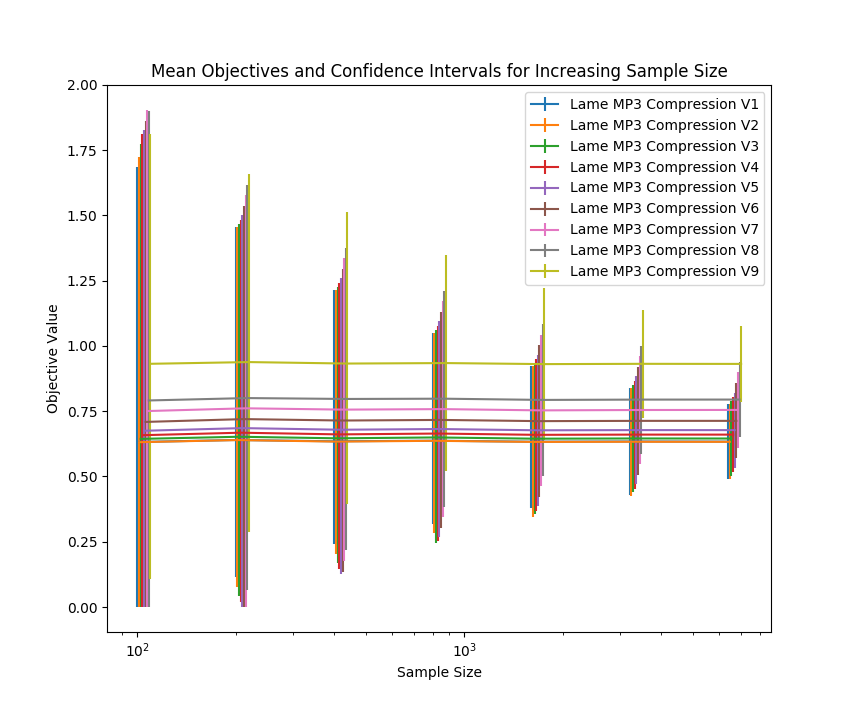
\includegraphics[width=4in]{codec_figures/obj1plot_py.png}
	\caption{Bounds on the objective $V_1(x) =   c_1(h(x)) + c_4(h(x))$ for each step of the PSP algorithm for audiobooks.}
	\label{obj1plot}
\end{figure}

\subsection{Tests on Audiobooks}

To test the model, we ran it on ten-second clips from open source audio books on LibriVox\citep{mcguire}. We collected over 25000 samples in that manner. When running the progressive sampling algorithm, we started by using 100 samples in the first round and doubling that quantity until terminating after 12800 samples were used on the eighth round. Notably, our algorithm did not actually isolate the best encoding function --- that would require more data. However, it succeeded in creating tight confidence intervals and in using those intervals to eliminate the worst function given our objective.

\todo{Run with more data to get better convergence}

\begin{figure}
    \centering
    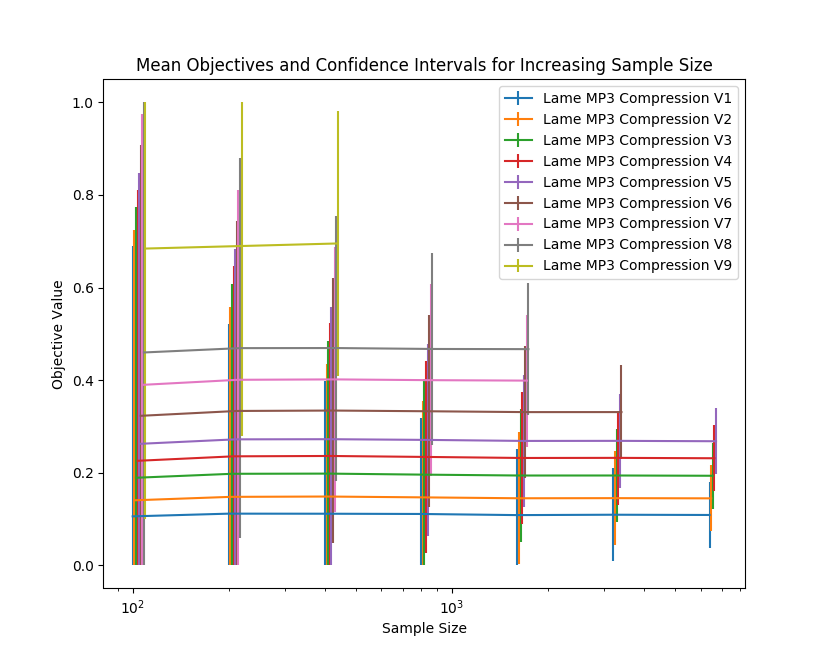
\includegraphics[width=4in]{codec_figures/obj2plot_py.png}
    \caption{Bounds on the objective $V_2(x) =  c_1(h(x))$ for each step of the PSP algorithm for audiobooks.}
    \label{obj2plot}
\end{figure}

Figure \ref{obj1plot} shows the empirical means and confidence intervals for the objective $V_1$ for each iteration and each compression scheme. While the means stay relatively stable, the bounds tighten with each iteration. Note that the V9 algorithm is eliminated after the seventh iteration because its confidence interval no longer intersects with the so-far optimal algorithm, V1. Given further iterations and more data, more algorithms could be eliminated as the bounds continue to tighten.

\begin{figure}
    \centering
    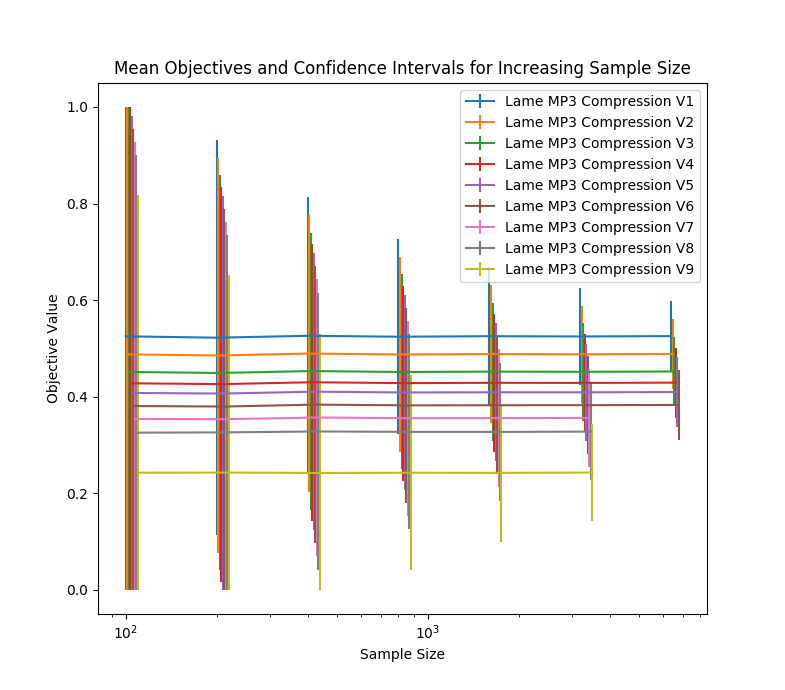
\includegraphics[width=4in]{codec_figures/obj3plot_py.png}
    \caption{Bounds on the objective $V_3(x) = c_4(h(x))$ for each step of the PSP algorithm for audiobooks.}
    \label{obj3plot}
\end{figure}

We can also visualize the bounds on our other proposed objectives. The difficulty of separating the performance of algorithms depends on the concentration of the objective values. In Figure \ref{obj2plot}, the empirical estimates of mean PEAQ divergence that comprise $V_2$ are very spread out, so the tightening bounds cease to overlap quickly. We can eliminate all but one suboptimal function this way. On the other hand, the estimates for $V_3$, which depends solely on compression ratio, in Figure \ref{obj3plot} are more concentrated near zero and therefore fail to ever obtain tight enough intervals to separate functions.

\subsection{Tests on Music}

We also tested the algorithm on small segments pulled from music files. The music dataset contains the complete orchestral works of Debussy, conducted by Yan Pascal Tortelier; the complete discography of hard rock band Led Zeppelin; and the 2000--2013 discography of progressive rock band Explosions in the Sky. We explored objectives over PEAQ divergence and compression ratios over a wider range of codecs; in addition to testing nine variants of VBR codecs, we also tested CBR codecs with fixed bit-rates of 320, 246, 128, and 64.

\begin{figure}
    \centering
    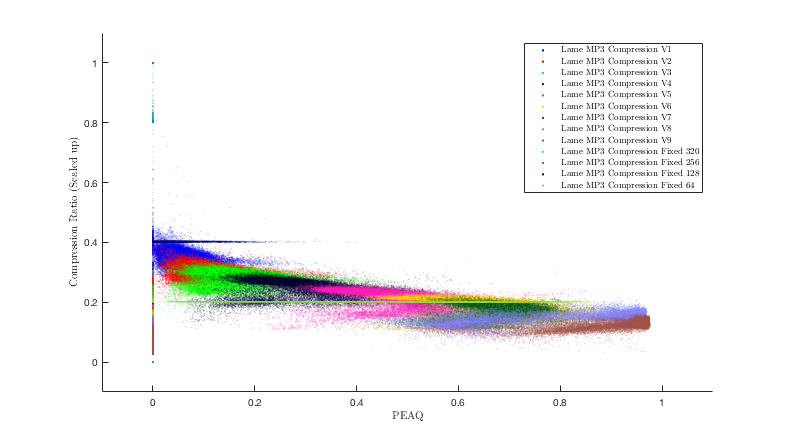
\includegraphics[width=\textwidth,trim={3cm 0 5cm 0},clip]{codec_figures/peaq_vs_cr_music2.png}
    \caption{A scatter-plot of scaled compression ratios versus PEAQ divergences for music segments when encoded by a wide range of codecs.}
    \label{peaq_cr}
\end{figure}

To visualize trends in these codecs, we compare PEAQ divergence and compression ratio in Figure \ref{peaq_cr}. Each point represents those criteria values for a sample encoded with a given function. Note that we scale up the compression ratio for this experiment in order to increase the variance of the metric without compromising accuracy; because WAV files are encoded at a bit-rate of 750 and because the highest bit-rate encoded by an MP3 is 320, we scaled each compression ratio by $\frac{750}{320}$ to spread out the data more while keeping all ratios within the interval $[0,1]$. We observe an inversely relationship with respect to compression ratio and PEAQ values as functions change. This makes sense because using more bits to encode a file leads to a smaller difference in sound between the original file and the decompressed file. Because they have fixed bit-rates, the CBR schemes have constant compression ratios, but vary widely in sound fidelity. The most accurate CBR schemes (256 and 320 bits) have zero perceived difference between the input and output files, but they have very high compression ratios.

\todo{Remake Figure 4}

\begin{figure}
    \centering
    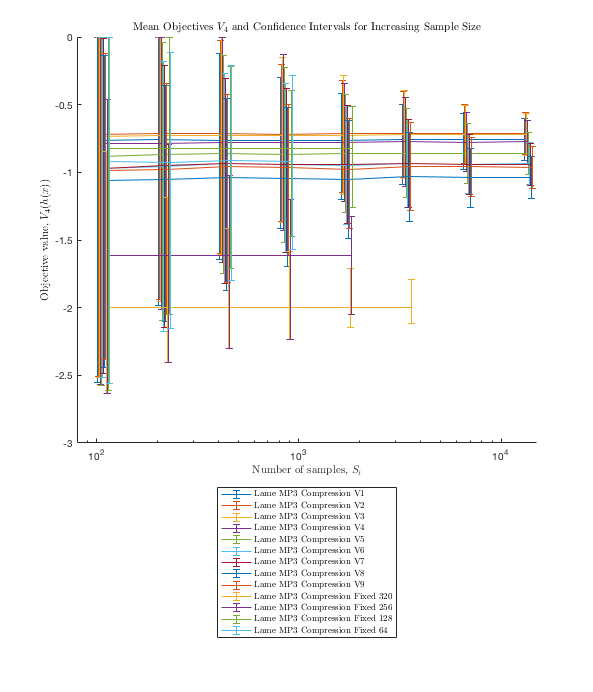
\includegraphics[width=\textwidth,trim={1.3cm 1.5cm 1.65cm 0.5cm},clip]{codec_figures/obj4plot.png}
    \caption{Bounds on the objective $V_4(x) = c_1(h(x)) + 2c_4(h(x))$ for each step of the PSP algorithm for music.}
    \label{obj4plot}
\end{figure}

In this more complicated case, we chose an objective that balances compression ratios and PEAQ divergences to choose a codec that effectively trades off between the two and does not simply maximize one of them. With the objective, $V_4(x) =   c_1(h(x))+ 2 c_4(h(x))$, we can quickly eliminate codecs like the CBRs with bit-rates 320 and 256, as shown in Figure \ref{obj4plot}. The VBR encoding scheme V2 emerges as the scheme that best trades off compression ratio and PEAQ, although it struggles to rule out other schemes because the trade off between the two criteria leads to similar objective values across a range of codecs.

For future experiments, we can use more data points to shrink the bounds further, to eliminate more compression algorithms, and to find the optimal encoding function with high certainty. We can additionally accelerate the rate of elimination by choosing more metrics like PEAQ that have significant differences in values for each compression function and incorporating them into the objective function. We also will test the audiobook data on a CBR codecs and compare those results to that of the music data on the balanced objective.

\subsection{Comparison with Approximate Bounds}
\todo{Add comparisons and figures}

\section{Discussion and Open Questions}
The PSP algorithm provides a clean application of uniform convergence bounds. Notably, instead of using the bounds to bound the accuracy of our results, we actually use them in an online manner while running the algorithm --- the bounds themselves determine the actions of the algorithm. We proved theoretical results that ensure the convergence of our algorithm, and we showed that the framework can be successfully applied to the domain of audio compression. However, no special characteristics of audio data are used here, so we could easily extend this to other function selection tasks.

We also hope to incorporate a broader range of criteria; in particular, we want to integrate criteria which synthesizes a range of feedback. For example, in the audio domain the similarity between two files is often measured \textit{subjectively} by human listener-provided ratings. Because perceptual abilities varies by listeners, we want to evaluate the listeners as well as the audio files. To do so, we can regard each data point as the pairing of a file and a listener, rather than just a file. We need a different method of complexity that allows samples to drawn with i.i.d. \textit{components}, even if the final samples are not i.i.d. The Cartesian EMD framework of \cite{cousins} is such a measure.

\subsubsection*{Acknowledgments}

\bibliographystyle{plainnat}%Used BibTeX style is unsrt
\bibliography{bib}


\end{document}
